\uuid{x8fv}
\exo7id{5665}
\titre{exo7 5665}
\auteur{rouget}
\organisation{exo7}
\datecreate{2010-10-16}
\isIndication{false}
\isCorrection{true}
\chapitre{Réduction d'endomorphisme, polynôme annulateur}
\sousChapitre{Applications}
\module{Algèbre}
\niveau{L2}
\difficulte{}

\contenu{
\texte{
Soit $A=(a_{i,j})_{1\leqslant i,j\leqslant n}\in\mathcal{M}_n(\Rr)$ telle que $\forall(i,j)\in\llbracket1,n\rrbracket^2,\;a_{i,j}\in[0,1]$ et $\forall i\in\llbracket1,n\rrbracket$, $\sum_{j=1}^{n}a_{i,j}= 1$.
}
\begin{enumerate}
    \item \question{Montrer que $1$ est valeur propre de $A$.}
\reponse{Les hypothèses fournissent $AU= U$ où $U=\left(
\begin{array}{c}
1\\
\vdots\\
1
\end{array}
\right)$ et donc $1$ est valeur propre de $A$.}
    \item \question{Soit $\lambda$ une valeur propre de $A$.
  \begin{enumerate}}
\reponse{\begin{enumerate}}
    \item \question{Montrer que $|\lambda|\leqslant 1$.}
\reponse{Soient $\lambda$ une valeur propre de $A$ et $X =\left(
\begin{array}{c}
x_1\\
\vdots\\
x_n
\end{array}
\right)\in M_{n,1}(\Cc)$ un vecteur propre associé.

\begin{align*}\ensuremath
AX =\lambda X&\Rightarrow\forall i\in\llbracket1,n\rrbracket,\;\sum_{j=1}^{n}a_{i,j}x_j=\lambda x_i\Rightarrow\forall i\in\llbracket1,n\rrbracket,\;|\lambda x_i|\leqslant\sum_{j=1}^{n}|a_{i,j}||x_j|\\
 &\Rightarrow\forall i\in\llbracket1,n\rrbracket,\;|\lambda x_i|\leqslant\left(\sum_{j=1}^{n}a_{i,j}\right)\text{Max}\{|x_j|,\;1\leqslant j\leqslant n\}\\
 &\Rightarrow\forall i\in\llbracket1,n\rrbracket,\;|\lambda| |x_i|\leqslant\text{Max}\{|x_j|,\;1\leqslant j\leqslant n\}.
\end{align*}

On choisit alors pour $i$ un indice $i_0$ tel que $|x_{i_0}|=\text{Max}\{|x_j|,\;1\leqslant j\leqslant n\}$. Puisque $X$ est non nul, on a $|x_{i_0}|> 0$. On obtient

\begin{center}
$|\lambda| |x_{i_0}|\leqslant|x_{i_0}|$ et donc $|\lambda|\leqslant 1$ puisque $|x_{i_0}| > 0$.
\end{center}}
    \item \question{Montrer qu'il existe un réel $\omega$ de $[0,1]$ tel que $|\lambda-\omega|\leqslant 1-\omega$. Conséquence géométrique ?}
\reponse{Plus précisément,

\begin{center}
$|\lambda-a_{i_0,i_0}||x_{i_0}|=\left|\sum_{j\neq i_0}^{}a_{i_0,j}x_j\right|\leqslant\sum_{j\neq i_0}^{}a_{i_0,j}|x_j|\leqslant \left(\sum_{j\neq i_0}^{}a_{i_0,j}\right)|x_{i_0}|=(1-a_{i_0,i_0})|x_{i_0}|$
\end{center}

et donc $\forall\lambda\in\text{Sp}A,\;|\lambda-a_{i_0,i_0}|\leqslant1-a_{i_0,i_0}$ ce qui signifie que les valeurs propres de $A$ appartiennent au disque de centre $a_{i_0,i_0}$ et de rayon $1-a_{i_0,i_0}$. Ce disque est tangent intérieurement au cercle de centre $(1,0)$ et de rayon $1$ en le point $(1,0)$.


$$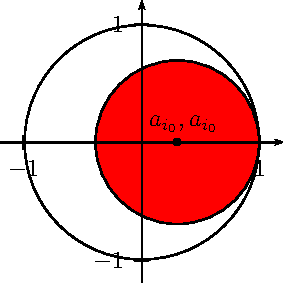
\includegraphics{../images/pdf/x8fv-1.pdf}$$}
\end{enumerate}
}
